\documentclass{article}

\usepackage{fontspec}   %加這個就可以設定字體
\usepackage{xeCJK}       %讓中英文字體分開設置
\usepackage[T1]{fontenc}
\usepackage{bigfoot} % to allow verbatim in footnote
\usepackage[numbered,framed]{matlab-prettifier}
\usepackage{graphicx}
\usepackage{filecontents}
\graphicspath{ {img/} }
\setCJKmainfont{標楷體} %設定中文為系統上的字型,而英文不去更動,使用原TeX字型
\XeTeXlinebreaklocale "zh"             %這兩行一定要加,中文才能自動換行
\XeTeXlinebreakskip = 0pt plus 1pt     %這兩行一定要加,中文才能自動換行
\title{Introduction to Wireless and Mobile Networking\\ Homework \#3}
\author{B03901023 許秉鈞}
\date{April 30, 2017} %日期
\let\ph\mlplaceholder % shorter macro
\lstMakeShortInline"

\lstset{
  style              = Matlab-editor,
  basicstyle         = \mlttfamily,
  escapechar         = ",
  mlshowsectionrules = true,
}

\begin{document}
\maketitle

\section{Please give a figure to describe how you arrange cell IDs to Fig. 1.}
\begin{figure}[h]
    \centering
    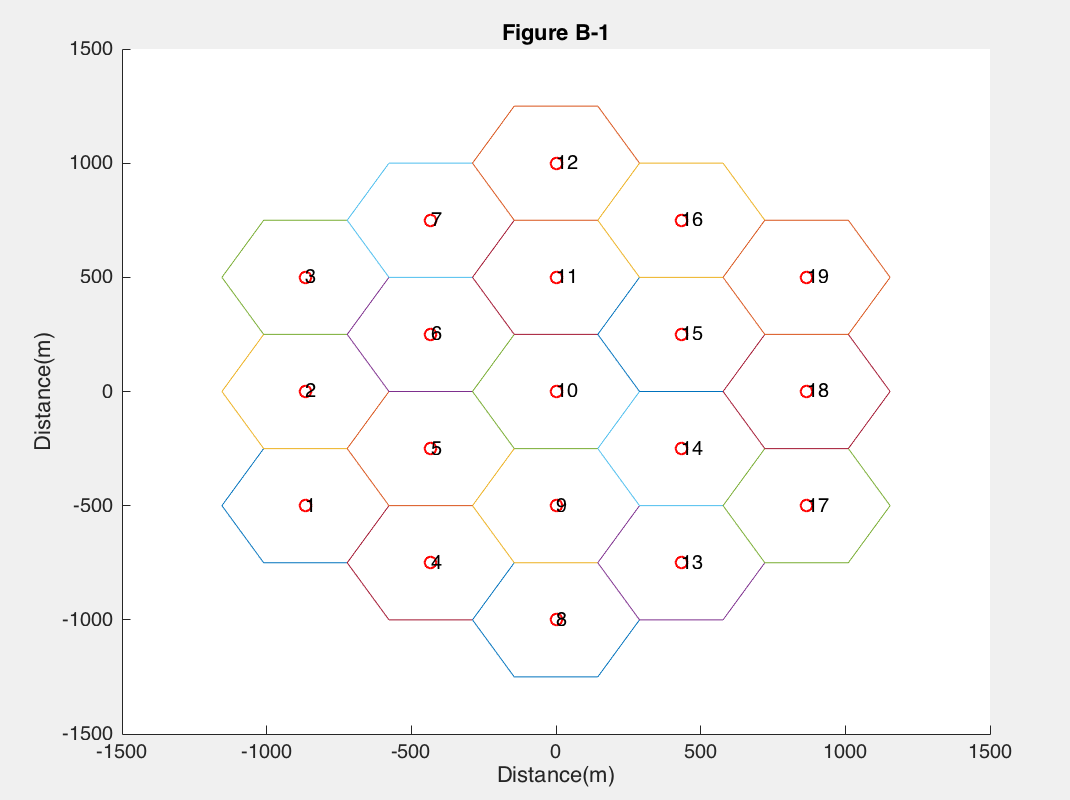
\includegraphics[width=1\textwidth]{fig1}
    \caption{\emph{B-1. Please give a figure to describe how you arrange cell IDs.}}
    \label{fig:mesh1}
\end{figure}



Please check the file \emph{mobile\_map.m}. The program will automatically generates the boundaries, which was called by the function \emph{hexagon\_v()} in line 16. To describe it briefly, first, I made those hexagons in the center, for which their \emph{baseX}, \emph{baseY} are all zeros.

\pagebreak

\begin{lstlisting}[caption = {mobile\_map.m}]
function [maxX, maxY, vX, vY] = mobile_map(X, Y, baseX, baseY, is_text, is_draw)
    dist = 500;
    side = dist/sqrt(3);
    bs_x = X + baseX;
    bs_y = Y + baseY;
    %init
    [v_x{1}, v_y{1}] = hexagon_v(side, bs_x(1), bs_y(1), is_draw);
    if is_text == 1
        text(bs_x(1), bs_y(1), int2str(1));
    end
    vX = v_x{1};
    vY = v_y{1};
    %put data
    for i = 2:19
        [v_x{i}, v_y{i}] = hexagon_v(side, bs_x(i), bs_y(i), is_draw);
        if is_text == 1
            text(bs_x(i), bs_y(i), int2str(i));
        end
        [vX, vY] = polybool('union', vX, vY, v_x{i}, v_y{i});
    end
    maxX = max(vX);
    maxY = max(vY);
end
\end{lstlisting}
The order of those 19 cells' IDs are as the following: 1st cell in the left-bottom, and then continuously grows from the left to right, bottom to top.
\pagebreak


\section{Please plot a map with all mobile devices in their initial location.}
\begin{figure}[h]
    \centering
    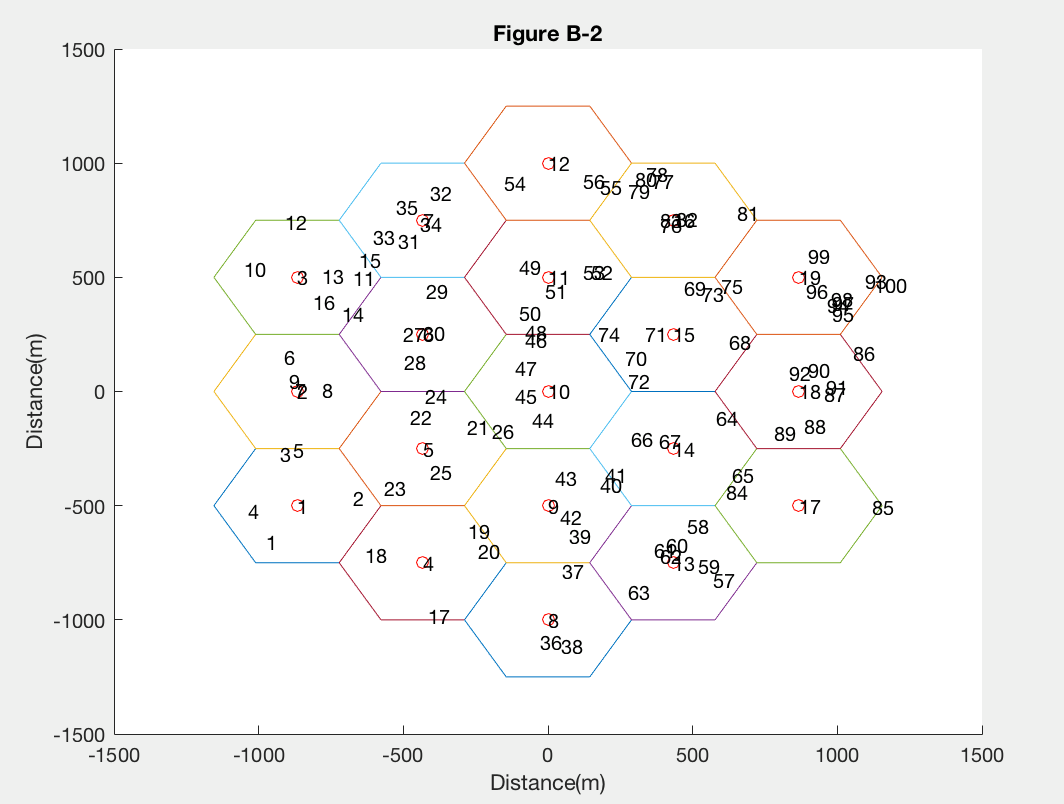
\includegraphics[width=1\textwidth]{fig2}
    \caption{\emph{B-2. Please plot a map with all mobile devices in their initial location.}}
    \label{fig:mesh2}
\end{figure}

\textbf{Describe how you decide the initial location.}

please check the following code(\emph{hw3\_bonus.m}) below. In line 37 to 50, The for loop runs cell\_num = 19 times, and after that we get the \emph{posX, posY} vectors represented the position of those surrounding points, which was defined in the function \emph{hexagon\_c.m}, the line 3 to 20. We will go through the process by the following function call as listed.
\begin{lstlisting}[caption = {hw3\_bonus.m}]
%% B-2. Please plot a map with all mobile devices in their initial location.
hold on;
myrand = randi( cell_num, [1, ms_num] );
for i = 1:cell_num
    mysum = sum(myrand == i);
    if mysum > 0
        [x, y] = hexagon_c(bs_x(i), bs_y(i), mysum);
        posX{i} = x;
        posY{i} = y;
    end
end
title('Figure B-1');
xlabel('Distance(m)'), ylabel('Distance(m)');
hold off;
\end{lstlisting}

\begin{lstlisting}[caption = {hexagon\_c.m}]
function [c_x, c_y] = hexagon_c(x0, y0, ms_num)
    dist = 500;
    N = ms_num; %ms_num = 100, Number of users
    R = dist/sqrt(3); %Radius of Hexagon
    v_x = R * cos((0:6)*pi/3);
    v_y = R * sin((0:6)*pi/3);
    %The method used here is to generate many points in a square and choose N points that fall within the hexagon
    %Generate 3N random points with square that is 2R by 2R
    c_x = R-rand(1, 3*N)*2*R; c_y = R-rand(1, 3*N)*2*R;
    %There is a command in MATLAB inploygon.
    %The command finds points within a polygon region. %get the points within the polygon
    IN = inpolygon(c_x + x0, c_y + y0, v_x + x0, v_y + y0);
    %drop nodes outside the hexagon
    c_x = c_x(IN); c_y = c_y(IN);
    %choose only N points
    idx = randperm(N);
    c_x = c_x(idx(1:N)) + x0;
    c_y = c_y(idx(1:N)) + y0;
end
\end{lstlisting}


\end{document}
